\documentclass[journal,12pt,twocolumn]{IEEEtran}
\usepackage{amsthm}
\allowbreak
\usepackage{setspace}
\usepackage{gensymb}
\singlespacing
\usepackage[cmex10]{amsmath}
\usepackage{caption}
\usepackage{amsthm}
\usepackage{float}

\DeclareUnicodeCharacter{2212}{-}
\usepackage{tikz}
\usepackage{pgfplots}

\usepackage{mathrsfs}
\usepackage{txfonts}
\usepackage{stfloats}
\usepackage{bm}
\usepackage{cite}
\usepackage{cases}
\usepackage{subfig}

\usepackage{longtable}
\usepackage{multirow}

\usepackage{enumitem}
\usepackage{mathtools}
\usepackage{steinmetz}
\usepackage{tikz}
\usepackage{circuitikz}
\usepackage{verbatim}
\usepackage{tfrupee}
\usepackage[breaklinks=true]{hyperref}
\usepackage{graphicx}
\usepackage{tkz-euclide}
\graphicspath{ {./images/} }
\usetikzlibrary{calc,math}
\usepackage{listings}
\usepackage{color}                                            %%
\usepackage{array}                                            %%
\usepackage{longtable}                                        %%
\usepackage{calc}                                             %%
\usepackage{multirow}                                         %%
\usepackage{hhline}                                           %%
\usepackage{ifthen}                                           %%
\usepackage{lscape}     
\usepackage{multicol}
\usepackage{chngcntr}

\DeclareMathOperator*{\Res}{Res}



\hyphenation{op-tical net-works semi-conduc-tor}
\def\inputGnumericTable{}                                 %%

\lstset{
	%language=C,
	frame=single, 
	breaklines=true,
	columns=fullflexible
}

\begin{document}
	
	\newcommand{\BEQA}{\begin{eqnarray}}
		\newcommand{\EEQA}{\end{eqnarray}}
	\newcommand{\define}{\stackrel{\triangle}{=}}
	\bibliographystyle{IEEEtran}
	\raggedbottom
	\setlength{\parindent}{0pt}
	\providecommand{\mbf}{\mathbf}
	\providecommand{\pr}[1]{\ensuremath{\Pr\left(#1\right)}}
	\providecommand{\qfunc}[1]{\ensuremath{Q\left(#1\right)}}
	\providecommand{\sbrak}[1]{\ensuremath{{}\left[#1\right]}}
	\providecommand{\lsbrak}[1]{\ensuremath{{}\left[#1\right.}}
	\providecommand{\rsbrak}[1]{\ensuremath{{}\left.#1\right]}}
	\providecommand{\brak}[1]{\ensuremath{\left(#1\right)}}
	\providecommand{\lbrak}[1]{\ensuremath{\left(#1\right.}}
	\providecommand{\rbrak}[1]{\ensuremath{\left.#1\right)}}
	\providecommand{\cbrak}[1]{\ensuremath{\left\{#1\right\}}}
	\providecommand{\lcbrak}[1]{\ensuremath{\left\{#1\right.}}
	\providecommand{\rcbrak}[1]{\ensuremath{\left.#1\right\}}}
	\theoremstyle{remark}
	\newtheorem{rem}{Remark}
	\newcommand{\sgn}{\mathop{\mathrm{sgn}}}
	\providecommand{\abs}[1]{$\left\vert#1\right\vert$}
	\providecommand{\res}[1]{\Res\displaylimits_{#1}} 
	\providecommand{\norm}[1]{$\left\lVert#1\right\rVert$}
	%\providecommand{\norm}[1]{\lVert#1\rVert}
	\providecommand{\mtx}[1]{\mathbf{#1}}
	\providecommand{\mean}[1]{E$\left[ #1 \right]$}
	\providecommand{\fourier}{\overset{\mathcal{F}}{ \rightleftharpoons}}
	%\providecommand{\hilbert}{\overset{\mathcal{H}}{ \rightleftharpoons}}
	\providecommand{\system}{\overset{\mathcal{H}}{ \longleftrightarrow}}
	%\newcommand{\solution}[2]{\textbf{Solution:}{#1}}
	\newcommand{\solution}{\noindent \textbf{Solution: }}
	\newcommand{\cosec}{\,\text{cosec}\,}
	\providecommand{\dec}[2]{\ensuremath{\overset{#1}{\underset{#2}{\gtrless}}}}
	\newcommand{\myvec}[1]{\ensuremath{\begin{pmatrix}#1\end{pmatrix}}}
	\newcommand{\mydet}[1]{\ensuremath{\begin{vmatrix}#1\end{vmatrix}}}
	\makeatletter
	\makeatother
	\let\StandardTheFigure\thefigure
	\let\vec\mathbf
	\vspace{3cm}
	\title{AI1110: Assignment 2}
	\author{SADINENI ABHINAY - CS21BTECH11055}
	\maketitle
	\newpage
	\bigskip
	\renewcommand{\thefigure}{\theenumi}
	\renewcommand{\thetable}{\theenumi}
	\textbf{ICSE class 12 paper 2018}
\section{Question 20(a)} 
	Find the line of regression of y on x from the following table.
\begin{table}[H]
	\resizebox{\columnwidth}{!} {
		\begin{tabular}{|c|c|c|c|c|c|}
			\hline
        x &1 &2&3 & 4& 5 \\
         \hline
        y &7 & 6 & 5 &4 & 3\\
        \hline
		\end{tabular}
	}
\end{table}
		Hence, estimate the y value when x=6.
		
\textbf{Solution.}

Given the observations \\
\begin{align}
\myvec{x \\y }:
\vec{A}\myvec{1 \\7 },
\vec {B}\myvec{2 \\6 },
\vec {C}\myvec{3 \\5 },
 \vec {D}\myvec{4 \\4 },
\vec {E}\myvec{5 \\3 }
\end{align}
\begin{table}[H]
	\resizebox{\columnwidth}{!} {
		\begin{tabular}{|c|c|c|c|}
			\hline
			x & y & xy & $x^{2}$ \\
			\hline
			1 &  7 & 7  &1 \\
		
				2 &  6 & 12   &4 \\
			
				3 &  5 & 15  &9 \\
			
				4 &  4 & 16  &16 \\
			
				5 &  3 & 15  &25 \\
			\hline
			$\sum x=15$ &$\sum  y=25$ &$\sum xy=65$  &$\sum x^2=55$  \\
			\hline
		\end{tabular}
	}
\end{table}
Mean values and coefficent $b_{yx}$ :
\begin{align}
	\bar{x}&=\frac{15}{5}=3\\
	\bar{y}&=\frac{25}{5}=5\\
	b_{yx} &=\frac{\sum xy - \frac{\sum x \sum y}{n}}{\sum x^{2}- \frac {\brak{\sum x}^{2}}{n} }\\
	&=\frac{65 -\frac{15.25}{5}}{55-\frac{225}{5}}\\
	&= -1 
\end{align}
The line of regression can be know from the form:
\begin{align}
	y-\bar{y}=b_{yx}\brak{x-\bar{x}}
\end{align}
so the line of regression in this problem:
\begin{align}
	y-5&=-1\brak{x-1} \\
	y-5&=3-x\\
	x+y&=8
\end{align}
When $x=6$ then y must be 2 from the line of regression.

\begin{figure}[h!]
		\centering
	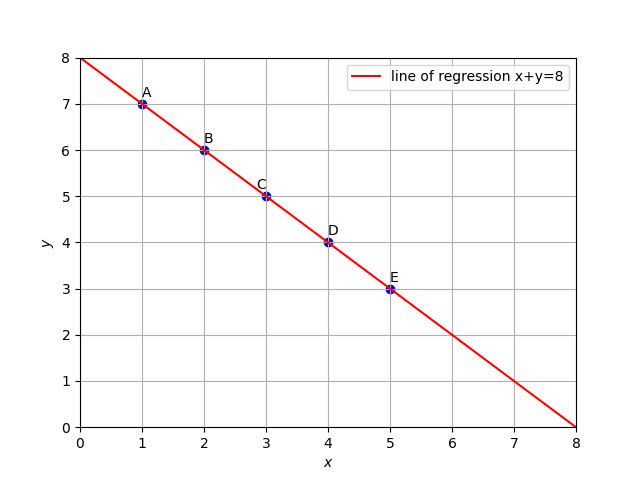
\includegraphics[width=\columnwidth]{./figs/fig1.png}
	\caption{plot of all points}
	\label{Fig1}
	\end{figure}

\end{document}